\documentclass{article}

% packages and stuff
\usepackage[utf8]{inputenc}
\usepackage[headheight = 18pt, footskip = 10pt]{geometry}
    \geometry{a4paper}
    \geometry{left=0.5in, right=0.5in, top=.95in, bottom=.95in}
\usepackage{graphicx}
\usepackage{amsmath}
%Better boxed command in math mode
\usepackage{empheq}
%Input text files and code
\usepackage{verbatim}
%Bold math
\usepackage{bm}
%Cancel to in math mode
\usepackage{cancel}
% Input standalone tex documents
\usepackage{standalone}
\usepackage{subcaption}
\usepackage{ulem}
\usepackage{bigstrut}
\usepackage{bm}
\usepackage{multirow}
\usepackage{calc}
\usepackage{xkeyval}
\usepackage{color, soul}
\usepackage{ifthen}
\usepackage{import}
\usepackage{times}
\usepackage{longtable}
\usepackage{tabularx}
\usepackage{multicol}
\usepackage{wrapfig}
\usepackage[font={small,it}]{caption}
\usepackage[version=4]{mhchem}
\usepackage{booktabs}

%New colors defined below
\definecolor{codegreen}{rgb}{0,0.6,0}
\definecolor{codegray}{rgb}{0.5,0.5,0.5}
\definecolor{codepurple}{rgb}{0.58,0,0.82}
\definecolor{backcolour}{rgb}{0.95,0.95,0.92}

% Include external pdf documents
\usepackage{pdfpages}

%Nice captions in floating figures
\usepackage{caption}

%%%%%%%%%%%%%%%%%%%%%%%%%%%%%%%%%%%%%%%%%%%%%%%%%%%%%%%%%%%%%%%%%%%%%%%%%%%%%%%%
\usepackage{fancyvrb}
\usepackage{comment}
\usepackage{enumerate}
\usepackage{subfiles}

%%%%%%%%%%%%%%%%%%%%%%%%%%%%%%%%%%%%%%%%%%%%%%%%%%%%%%%%%%%%%%%%%%%%%%%%%%%%%%%

% capital H is a champion
\usepackage{float}
    \restylefloat{table}

% make section styles non-lame
\usepackage{sectsty}
    \allsectionsfont{\mdseries\upshape}

% easy coloring for todo notes
\newcommand{\done}{\todo[inline, color=green]{(DONE)}{}}
\newcommand{\notdone}{\todo[inline, color=red]{(NOT DONE)}{}}
\newcommand{\fix}[1]{\todo[inline, color=red!75]{(FIX) #1}{}}
\newcommand{\discuss}[1]{\todo[inline, color=blue!40]{(DISCUSS) #1}{}}
\newcommand{\note}[1]{\todo[inline, color=yellow!20]{(NOTE) #1}}
\newcommand{\review}{\todo[inline, color=red!45!yellow!45]{(REVIEW)}{}}


\pagenumbering{gobble}
\setlength\parindent{10pt}
\setlength{\parskip}{0pt}
\setlength{\abovedisplayskip}{0pt}
\setlength{\belowdisplayskip}{0pt}
\relpenalty=10000 % don't split equations!!
\binoppenalty=10000 % don't split equations!!

\newcommand{\FigSiz}{0.37\textwidth}

% Set global figure size variable

\makeatletter
\define@key{Gin}{figsize}[true]{%
    \edef\@tempa{{Gin}{width=\FigSiz}}%
    \expandafter\setkeys\@tempa
}
\makeatother


%%%%%%%%%%%%%%%%%%%%%%%%%%%%%%%%%%%%%%%%%%%%%%%%%%%%%%%%%%%%%%%%%%%%%%%%%%%%%%%%%%%%%%%%%%%%%%%


% Custom title
\pagenumbering{arabic}
\usepackage{lastpage}
\usepackage{fancyhdr}
    \fancyhead{}
    \fancyfoot{}
    \pagestyle{fancy}
    \chead{\Large CS575: Project 4}
    \lhead{\Large Andrew Alferman}
    \rhead{\Large \today}
    \cfoot{\thepage  ~\ of ~\pageref{LastPage}}

\usepackage{titlesec}
\titlespacing*{\subsection}
{0pt}{0.65\baselineskip}{0.65\baselineskip}

%%%%%%%%%%%%%%%%%%%%%%%%%%%%%%%%%%%%%%%%%%%%%%%%%%%%%%%%%%%%%%%%%%%%%%%%%%%%%%%%%%%%%%%%%%%%%%%
\begin{document}



% Brief summary of the assignment
\begin{wrapfigure}{L}{0.25\textwidth}
        \begin{center}
        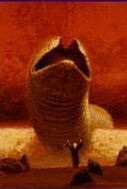
\includegraphics[width=0.15\textwidth]{Sandworm_heretics.jpg}
        \end{center}
        \caption{A sandworm.  Human shown in foreground for scale.}
        \label{fig:Sandworm}
\end{wrapfigure}
The purpose of this assignment was to 

Modifications to the original simulation included an increase in the number of deer to start out (20), with a corresponding increase in the grain height (30).  The reason for this is that the deer need a population of some size in order to sustain growth.  As one deer cannot reproduce by itself, a minimum of 2 deer are required to increase the population further.  The increase in the number of deer would eventually reach an equilibrium at a lower number of deer provided the same rate of grain consumption and growth, therefore to correct for these higher numbers, the amount of grain that one deer eats per month was reduced to 0.1 inch.

In addition to modifying these initial parameters, the average rainfall per month was made to be a float instead of a constant float for reasons that will soon become clear.  Finally, logic was added to ensure that the number of deer and the height of the grain could not ever be less than zero.

\subsection*{Question 1}
\textit{What was your own-choice quantity and how does it fit into the simulation.}

The quantity introduced into the simulation were sandworms inspired by the \textit{Dune} series of novels (see Figure \ref{fig:Sandworm}).  These enormous, ancient creatures are able to devour dozens of puny, helpless deer at once in its gaping mouth.  Sandworms do not have eyes, but they are very sensitive to noise.  This is a natural adaptation because their natural habitat is deep underground.  Occasionally, they breach the surface, consuming everything in their path, whether it be deer, grain, or rock.

Because of the large, indiscriminate nature of their feeding, each time a sandworm strikes it will consume large numbers of deer as well as a smaller quantity of grain.  Smaller populations of deer will cower in terror, spreading out so as to make less concentrated noise.  Because of this, the simulation is configured for the sandworms to eat fewer deer as the deer population gets smaller.  The trigger for a sandworm attack is four of consecutive months of growth in deer population.  Large numbers of young deer are inexperienced in their dealings with sandworms, and so they will make lots of noise.

As a quirk of the life cycle of the sandworm, the amount of water available on the planet will steadily decrease.  All this water will be brought deep underground by the larval stage of the sandworm, and there will be less precipitation.  Eventually, the planet will become a desert wasteland, void of all vegetation.  The deer must adapt by finding creative ways to conserve water and grow crops in isolated 

\subsection*{Question 2}
\textit{Show a table for temperature, precipitation, number of deer, height of the grain, and your own-choice quantity as a function of month number.}

\subsection*{Question 3}

\begin{wrapfigure}{C}{0.51\textwidth}
        \begin{center}
        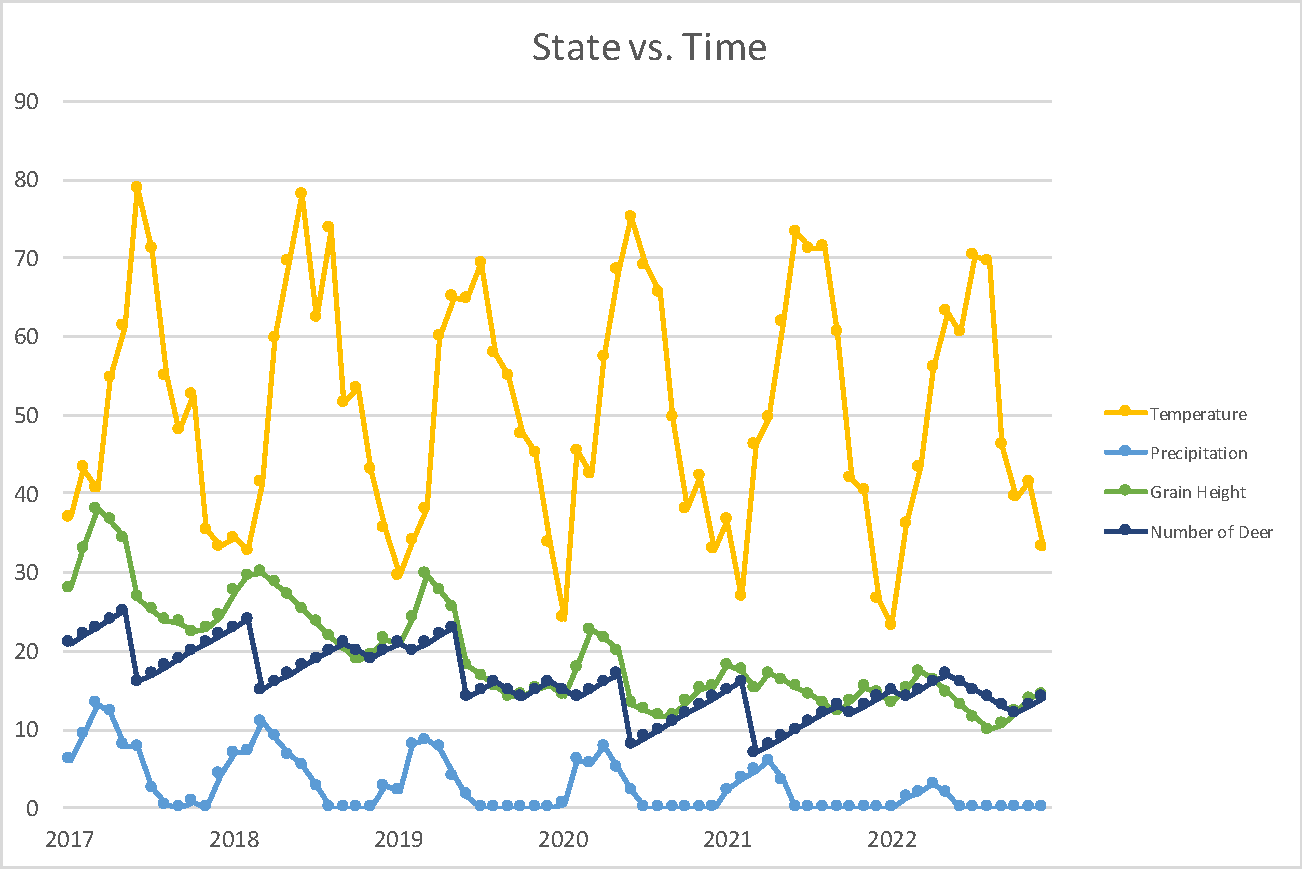
\includegraphics[width=0.5\textwidth]{Picture1.pdf}
        \end{center}
        \caption{State of the simulation over time.  Note the sharp declines in population that occur when sandworms strike.  As the population of deer get more experienced towards the end of the simulation, they learn to make less noise, attracting fewer sandworms.  Ultimately, however, they will be doomed unless they learn to conserve water.}
        \label{fig:State Plot}
\end{wrapfigure}

\subsection*{Question 4}

\subsection*{Question 5}

\newpage
\section*{Appendix}
\subsection*{Raw Data Used}

\end{document}
